\documentclass[12pt]{article}
\usepackage[utf8]{inputenc}
\usepackage[T1]{fontenc}
\usepackage{amsmath,amssymb,amsthm} % matematik
\usepackage{natbib}
\usepackage{titlesec}
\usepackage{setspace}
\usepackage[percent]{overpic}
\usepackage{tabularx}
\usepackage[flushleft]{threeparttable}
\usepackage{graphicx} % Allows including images
\usepackage{float}

\title{Social Data Science exam project}
\author{Group 9, Rasmus Gars, Lukas Hidan, Hjortur Hjartar and Mads Wulff Harslund}
\date{October 2015}


\makeatletter

\makeatother

\usepackage{caption}
\usepackage{subcaption}

\DeclareCaptionFormat{subfig}{\figurename~#1#2#3}
\DeclareCaptionSubType*{figure}
\captionsetup[subfigure]{format=subfig,labelsep=colon,labelformat=simple}



%\setlength\parindent{0pt}
\onehalfspacing
\usepackage[top=1.5in, bottom=1.5in, left=1in, right=1in]{geometry}
\usepackage{fancyhdr}

\begin{document}
\maketitle

	\section{Purpose} % (fold)
	\label{sec:problem_1}
	In this paper we examine a controversial subject - is the movie better than the book? By collecting and examining user-generated ratings of books and movies, we find that....

	However, there are also several important caveats when examining the data, which we discuss in the paper. 

	Normalisation 



\section{Data} % (fold)
	\label{sec:data}


The data collection is subject to a selection bias, which we will discuss later.
We consider ratings as a monotonic ordinal measure for quality of the medium. Comparing these ratings can be difficult, as we will discuss later.


\subsection{Movie ratings}
We collect data on movies from the site IMDb.com, which collects a variety of information  of 3,5572,200 titles (including TV-shows, documentaries, etc.) at the time of scraping on December 6th 2015. We collect data on a subset of the entire moviedatabase, namely those who are tagged as "based on novel". This amounts to 20,665 individual films. There are also tv-series and tv-films that are based on movies, but we do not include them.

We are especially interested in the rating of the movies, which is given on a scale of 1 to 10. We also collect the movie title and the number of votes given to the rating. There are some legal issues surrounding the collections of data, that we will discuss later.

IMDb states that their movies ratings are not pure arithmetic means of the ratings. They state that they make some adjustements in order to battle "vote stuffing", ie. inflating votes by rating several times through a computer farm in the Philippines. IMDb does not disclose the method they use to adjust the ratings in order to prevent abuse of it. We use the IMDb rating as it stated on a movie's page, as we believe it is more representative of the average IMDB user than the pure arithmetic mean.

All movies we collect data on are made after the book is published, such that there are no books made on movies. 

\subsection{Book ratings} % (fold)
\label{sub:book_ratings}
We collect data on books from the user-driven site Goodreads, which collects user-generated reviews on novels

We collect the user-generated rating which is given on a scale of 1 to 5. The rating is an arithmetic average of We also collect the book title and the number of votes given in the rating. 


\subsection{Merging book and movie data}
We merge the two data sets

This merging assumes that the title of the book and the movie are the same, which might not be the case. The different naming of books and movies can be made of artistic reasons or to avoid confusion or even trademark issues from other movies. As we merge a subset of movies and films that are stated as being based on books, we assume that the probability of a film not refering to the book of the same insignificant. Some books foster more than one movie based on it. We assume that due to naming and trademark rights, that movies with the same title are based on the same book.


Both subsets of the data are generated by users of the sites and may be subject to false data, unsincere ratings or outright trolling. Both sites have dedicated users, such that we hope that any false data is quickly deleted. 

As referred to above, the IMDb rating is not an arithmetic average, but the Goodreads rating is. We assume that Goodreads also make some effort to battle "vote stuffing"
\begin{table}[thb!]
\caption{Descriptive statistics of the rating variables}\label{tab:descr}
\begin{threeparttable}
\begin{tabular*}{\textwidth}{@{\extracolsep{\fill} }lrr}
\textbf{Measure} & \textbf{IMDb ratings} & \textbf{Goodread ratings} \\
\hline
Min & 2.6 & 2.85 \\  
Mean & 6.692 & 3.9  \\
Max & 9.2 & 4.5 \\
Mean Number of Ratings & 57,394 & 217,831 \\
Standard Deviation & 0.985 & 0.217 \\
Number of Observations & 878 & 878 \\
\hline
\end{tabular*}
\begin{tablenotes}
\footnotesize
\item \emph{Source: R-calculations on data scraped from imdb.com and goodreads.com}
\end{tablenotes}
\end{threeparttable}
\end{table}



\subsection{Making movie and book data comparable}
In our initial comparison naive comparison, we multiply the 5-star ratings of Goodreads by 2 in order to obatain a 10-star scale like IMDb's. Doing so, we plot the IMDb ratings against the doubled Goodreads ratings in figure \ref{fig:naive}. We thereby visualise how many 
\begin{figure}[H]
\centering
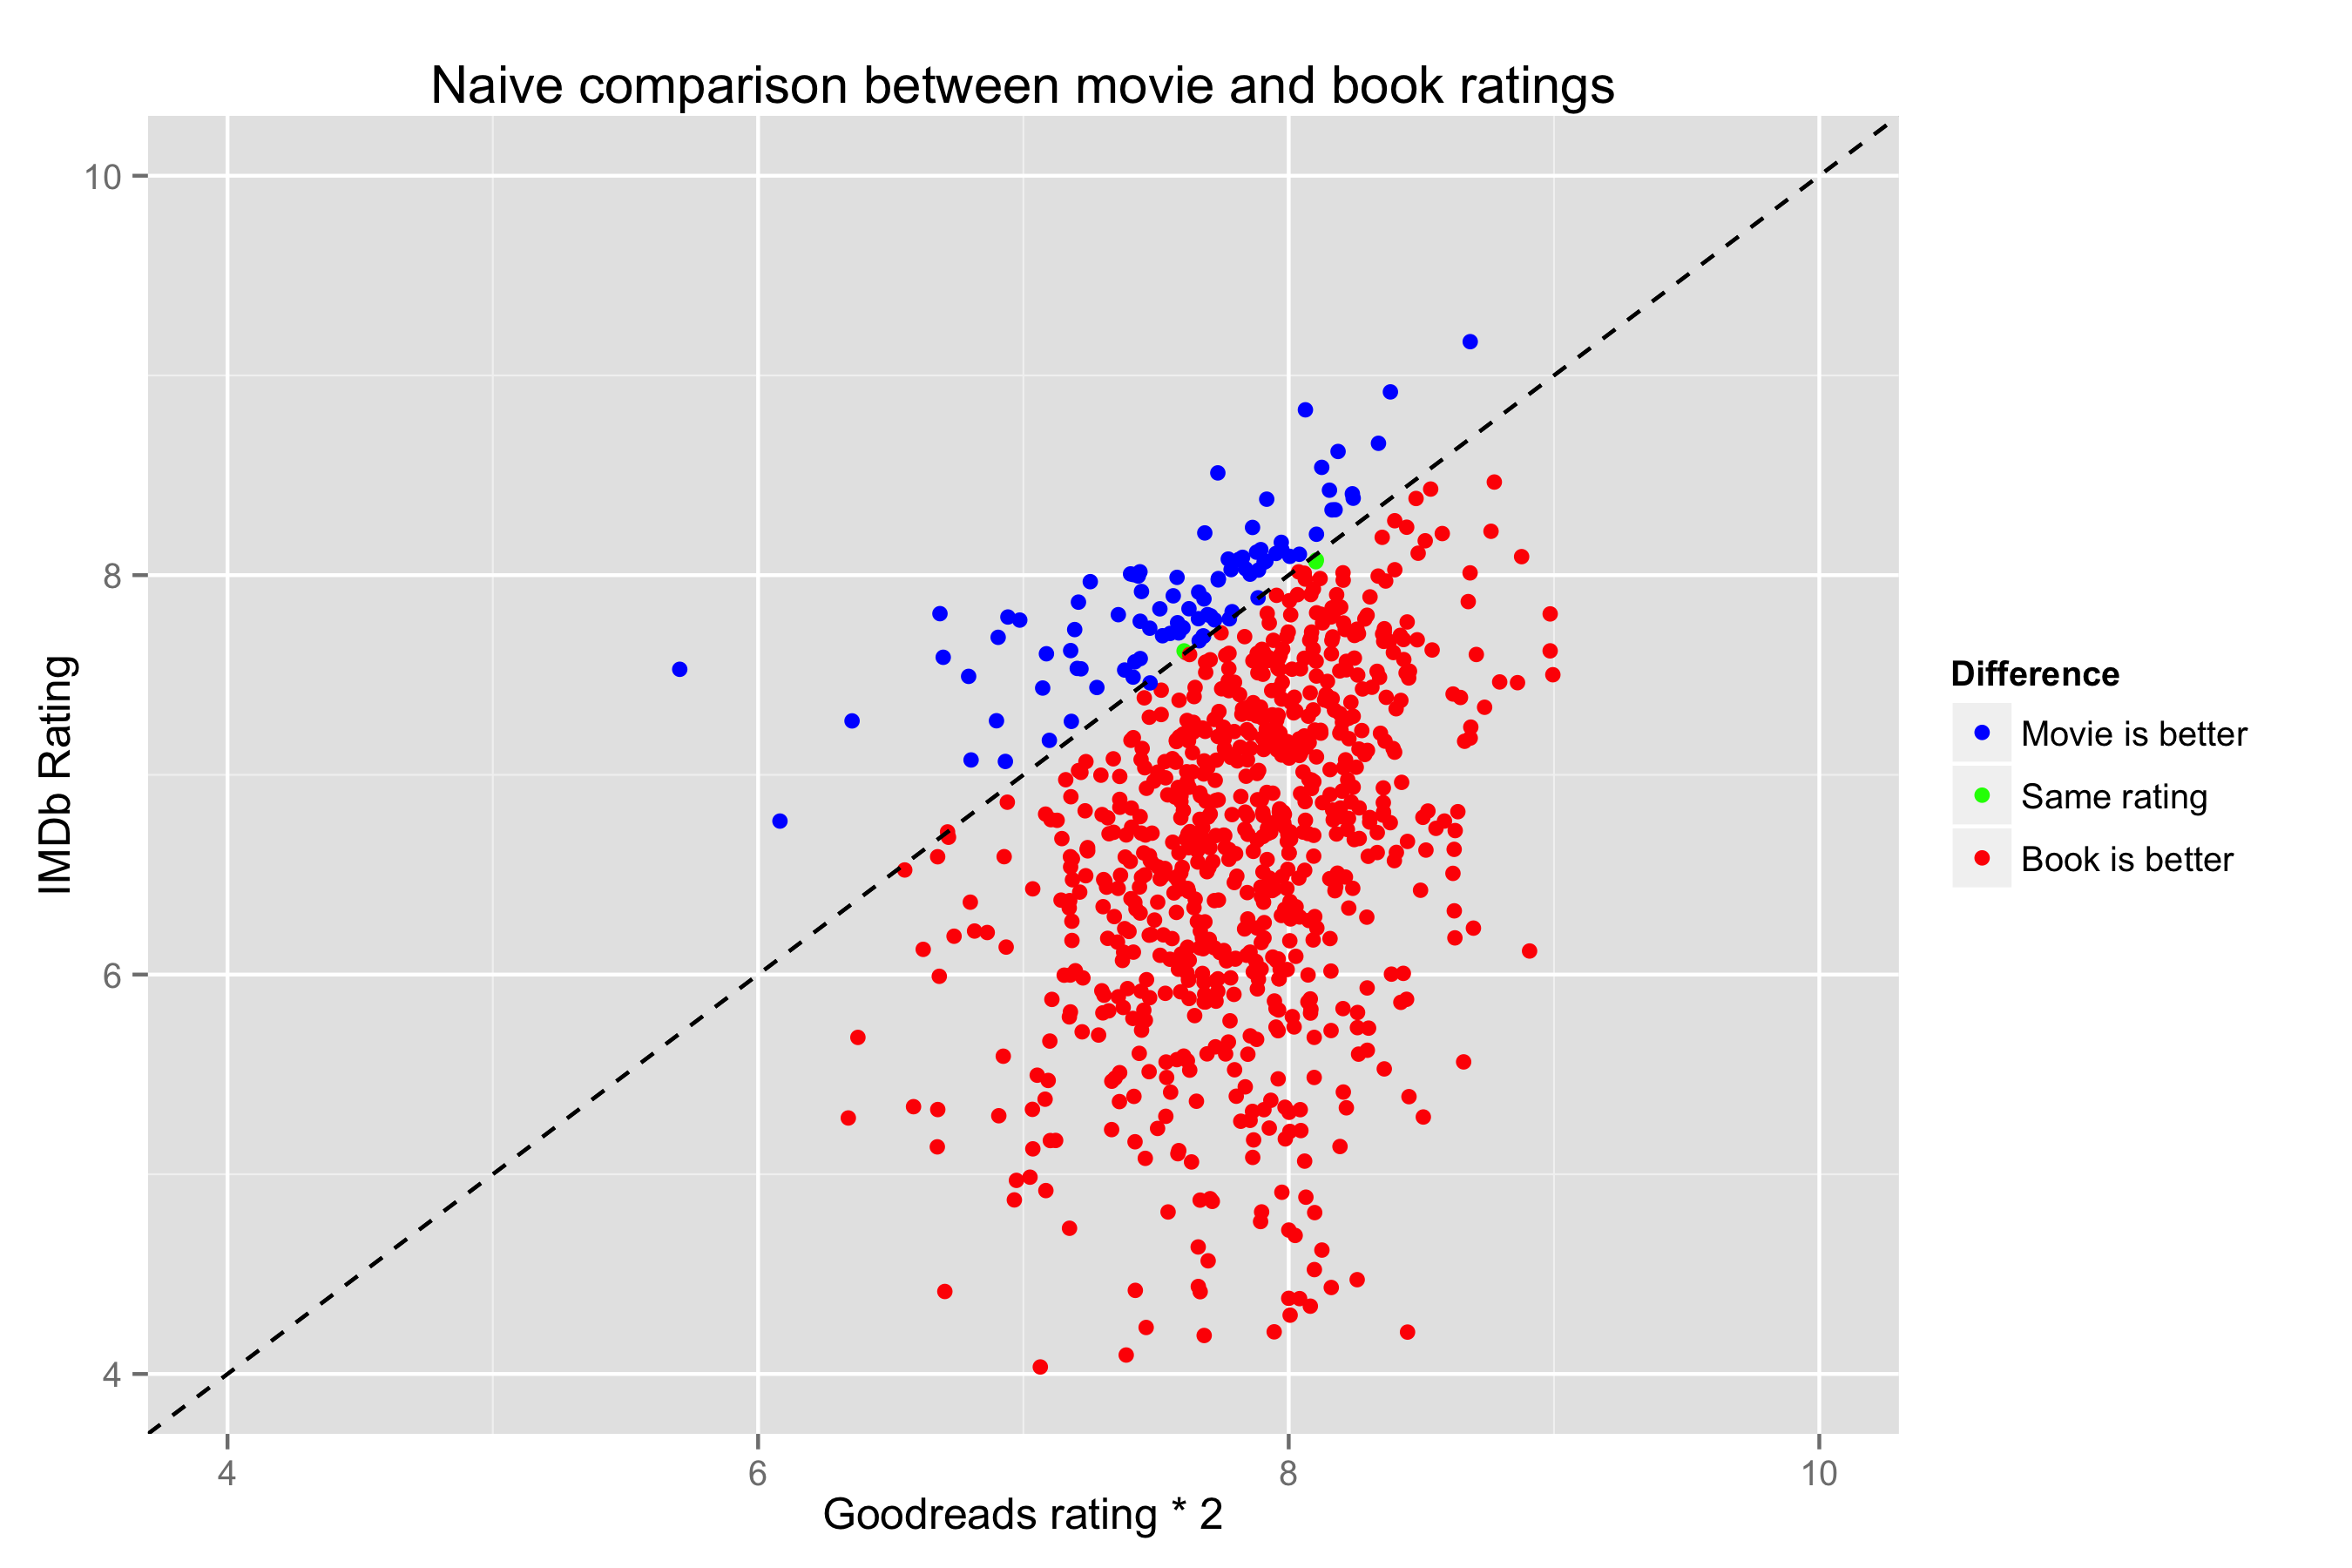
\includegraphics[scale=0.1]{naive}
\caption{\footnotesize Mean ratings for IMDb and Goodreads. Goodreads ratings are multiplied by 2 for comparison. The dotted diagonal line is a 45 degree line. The dots above this line (marked blue) represent movies that are better than  books, and dots below the line (marked red) represent books that are better}
\label{fig:naive}
\end{figure}
From figure \ref{fig:naive}, one could conclude that the majority of books are better than movoes

Clearly, the distribution of ratings are differently set. Comparing these two raw rating systems may therefore not give us a truthful picture of the relationship between book and movie ratings. 






\begin{figure}[H]
\centering
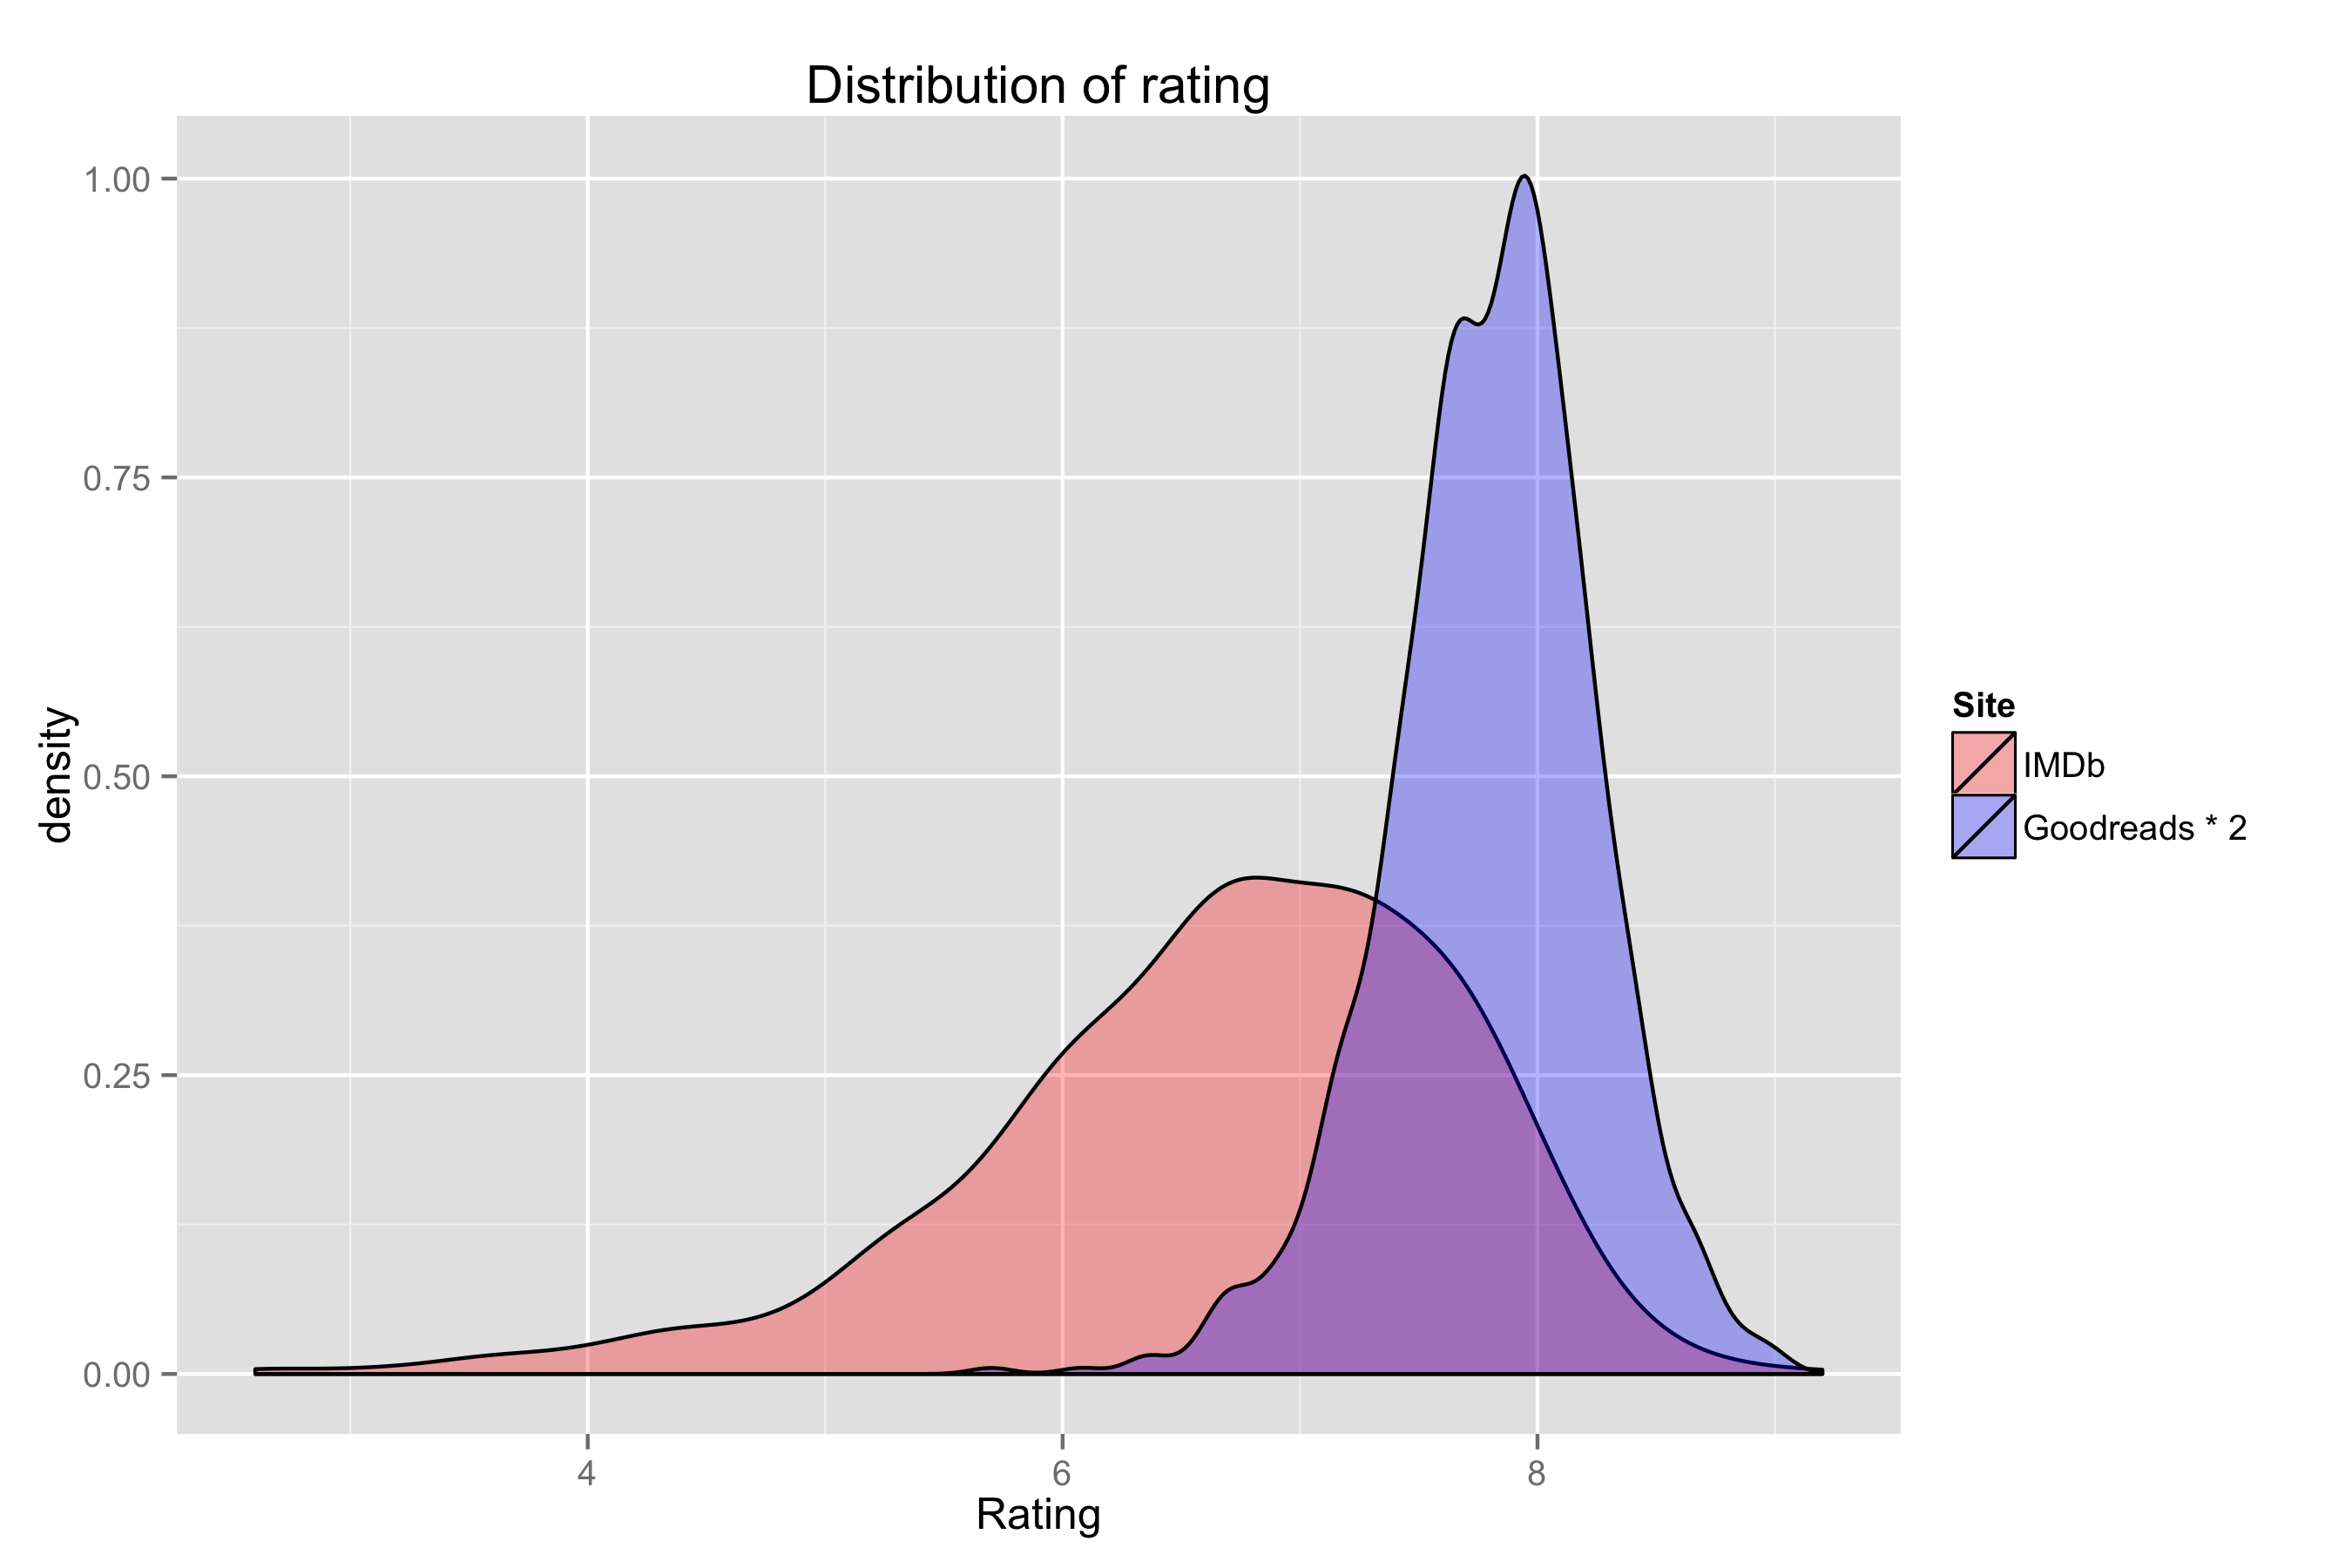
\includegraphics[scale=0.1]{rating}
\caption{Distribution of mean ratings for IMDb and Goodreads. Goodreads ratings are multiplied by 2 for comparison }
\label{fig:my_label}
\end{figure}






\section{Discussion} % (fold)
\label{sec:discussion}

% section discussion (end)

\subsection{Selection bias}

Since our data is built on books which were turned into a movie, some important things are worth noticing.
There is a strong argument for presence of selection bias, i.e. non-random selection. In this case it might be that some specific types of books are being included or left out of the sample in a non-random fashion, because they were turned into a movie.
In this case it is obvious to think that we have strong selection bias because only good, or above average, books were considered for a movie. A reasonable argument for this is that for a producer it should be more expected to have a willing audience if the back ground material (i.e. the book) already was popular.
At first it might therefore seem that the resulting movies cannot live up to the quality of the books but what we do not observe is how films, that were produced on the background of poorly rated books, would be rated. 

\subsection{Response bias}

One also need to understand who the voters are.  Looking closer at the web-pages in which we found the ratings, it might also be a very real possibility that we have a specific type of people voting on these pages. If for example a large share of people voting a Goodreads were between 20 and 35, it might explain the positive responses for e.g. the Harry Potter series, since these people grew up with the books.
A random sample of people would most likely not view e.g. the Harry Potter series as well as the people voting at Goodreads.
Since voting is voluntary, it is often suspected that overrepresentation of individuals with strong opinions takes place, voluntary response bias. I.e. mostly people who think the book/movie was really GOOD or really BAD will vote. This effect is probably made stronger due to the fact that people need to make an account to vote at both IMDb and Goodreads. This effectively acts as a barrier of entry for people who do not feel strongly about the subject. However when logged in, only the number of stars, i.e. rating, need to be clicked in order to vote on a subject of interest.
 And since giving a low rating to a book or movie with already high ratings does not matter a lot, many people with opposing views might be discouraged to vote, inflating the results towards either extremity.

\subsection{Expectations}

When people decide to vote, they often do so according to fulfilment of expectations. According to a study of hotels there is a negative correlation between expectations and ratings given. This might apply to the movies - since the books are highly rated, expectations are high, and as such, more movies, which in a non-context could be good, are rated below average. 

In the hotel study the authours suggest two explanations: Page 139
1.	The value gained from the product (here: movie) did not meet expectations which were formed from the reviews of other people. An overly high expectation would as such result in a down-wards driven user experience and therefore lower rating
2.	The value from the product did not seem to match the general rating and to help future users, the user would cast a rating which would go in the opposite direction of the present expectation. This explanation does not require the user himself to have expectations.


\subsection{Number of votes cast}

\begin{figure}[!ht]
  \begin{subfigure}[b]{.5\linewidth}
    \centering
    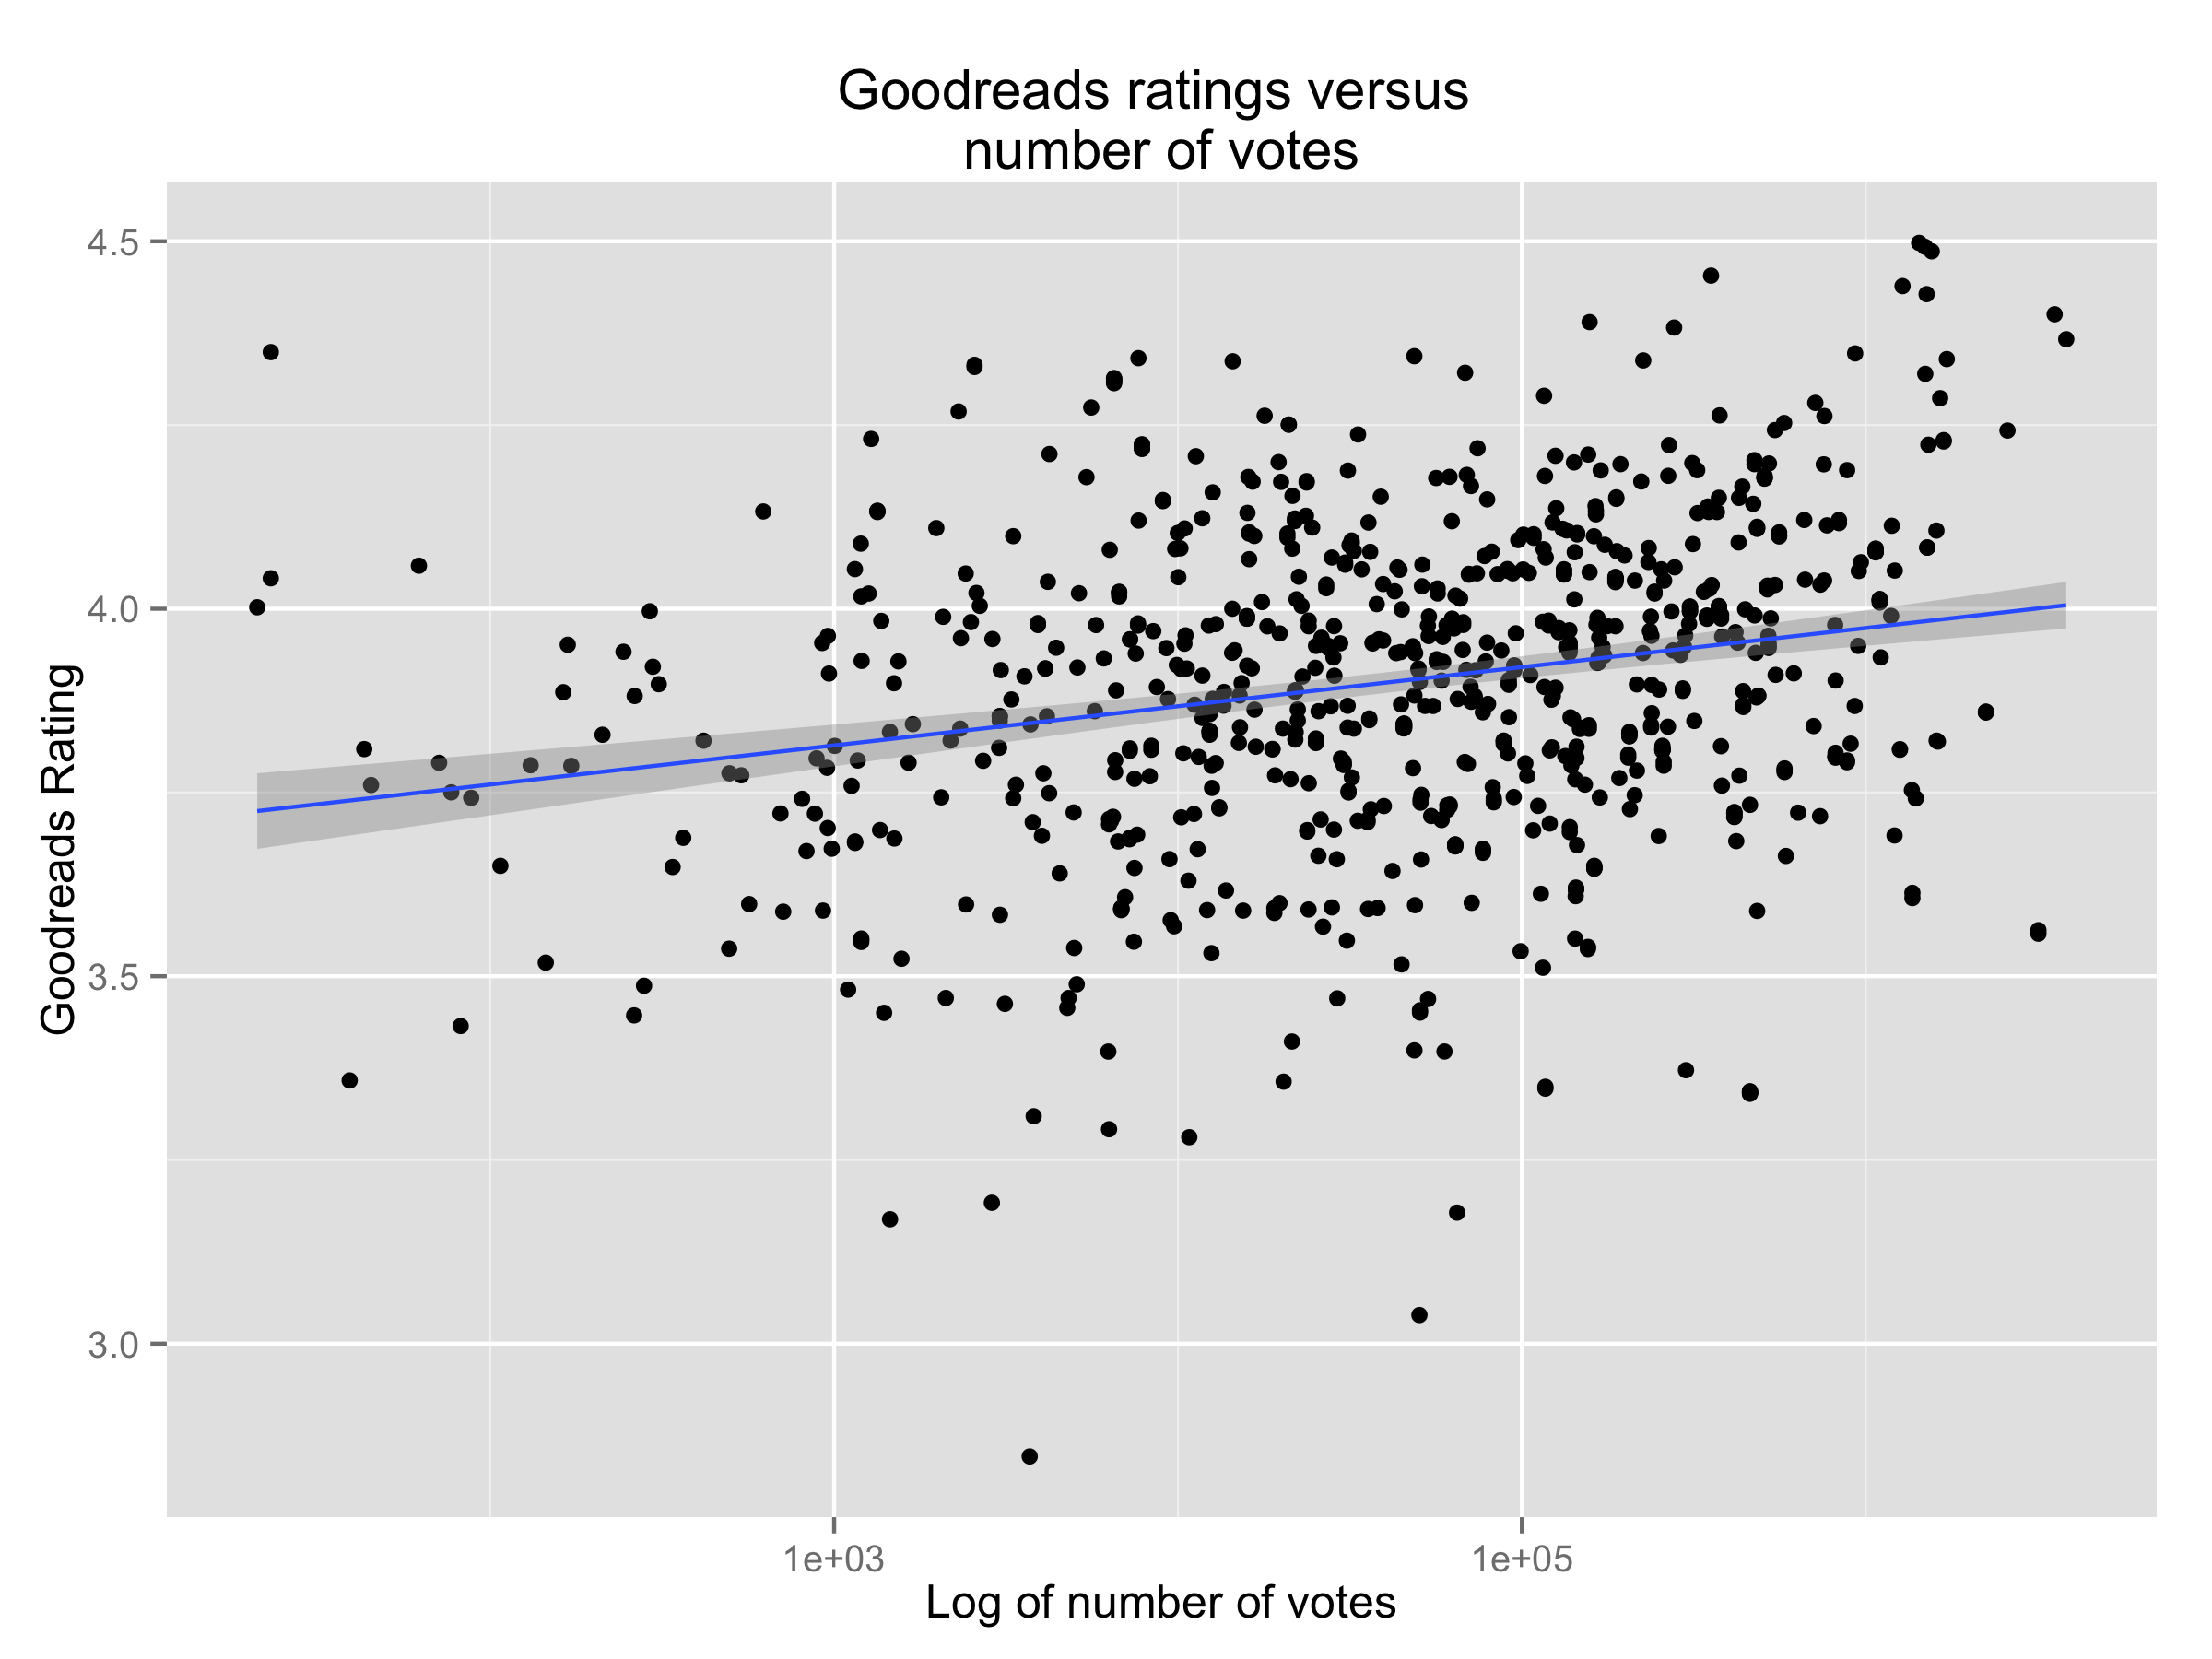
\includegraphics[scale=0.1]{ratingsbooks}
    \caption{Goodreads}
    \label{fig:1a}
  \end{subfigure}%
  \begin{subfigure}[b]{.5\linewidth}
    \centering
    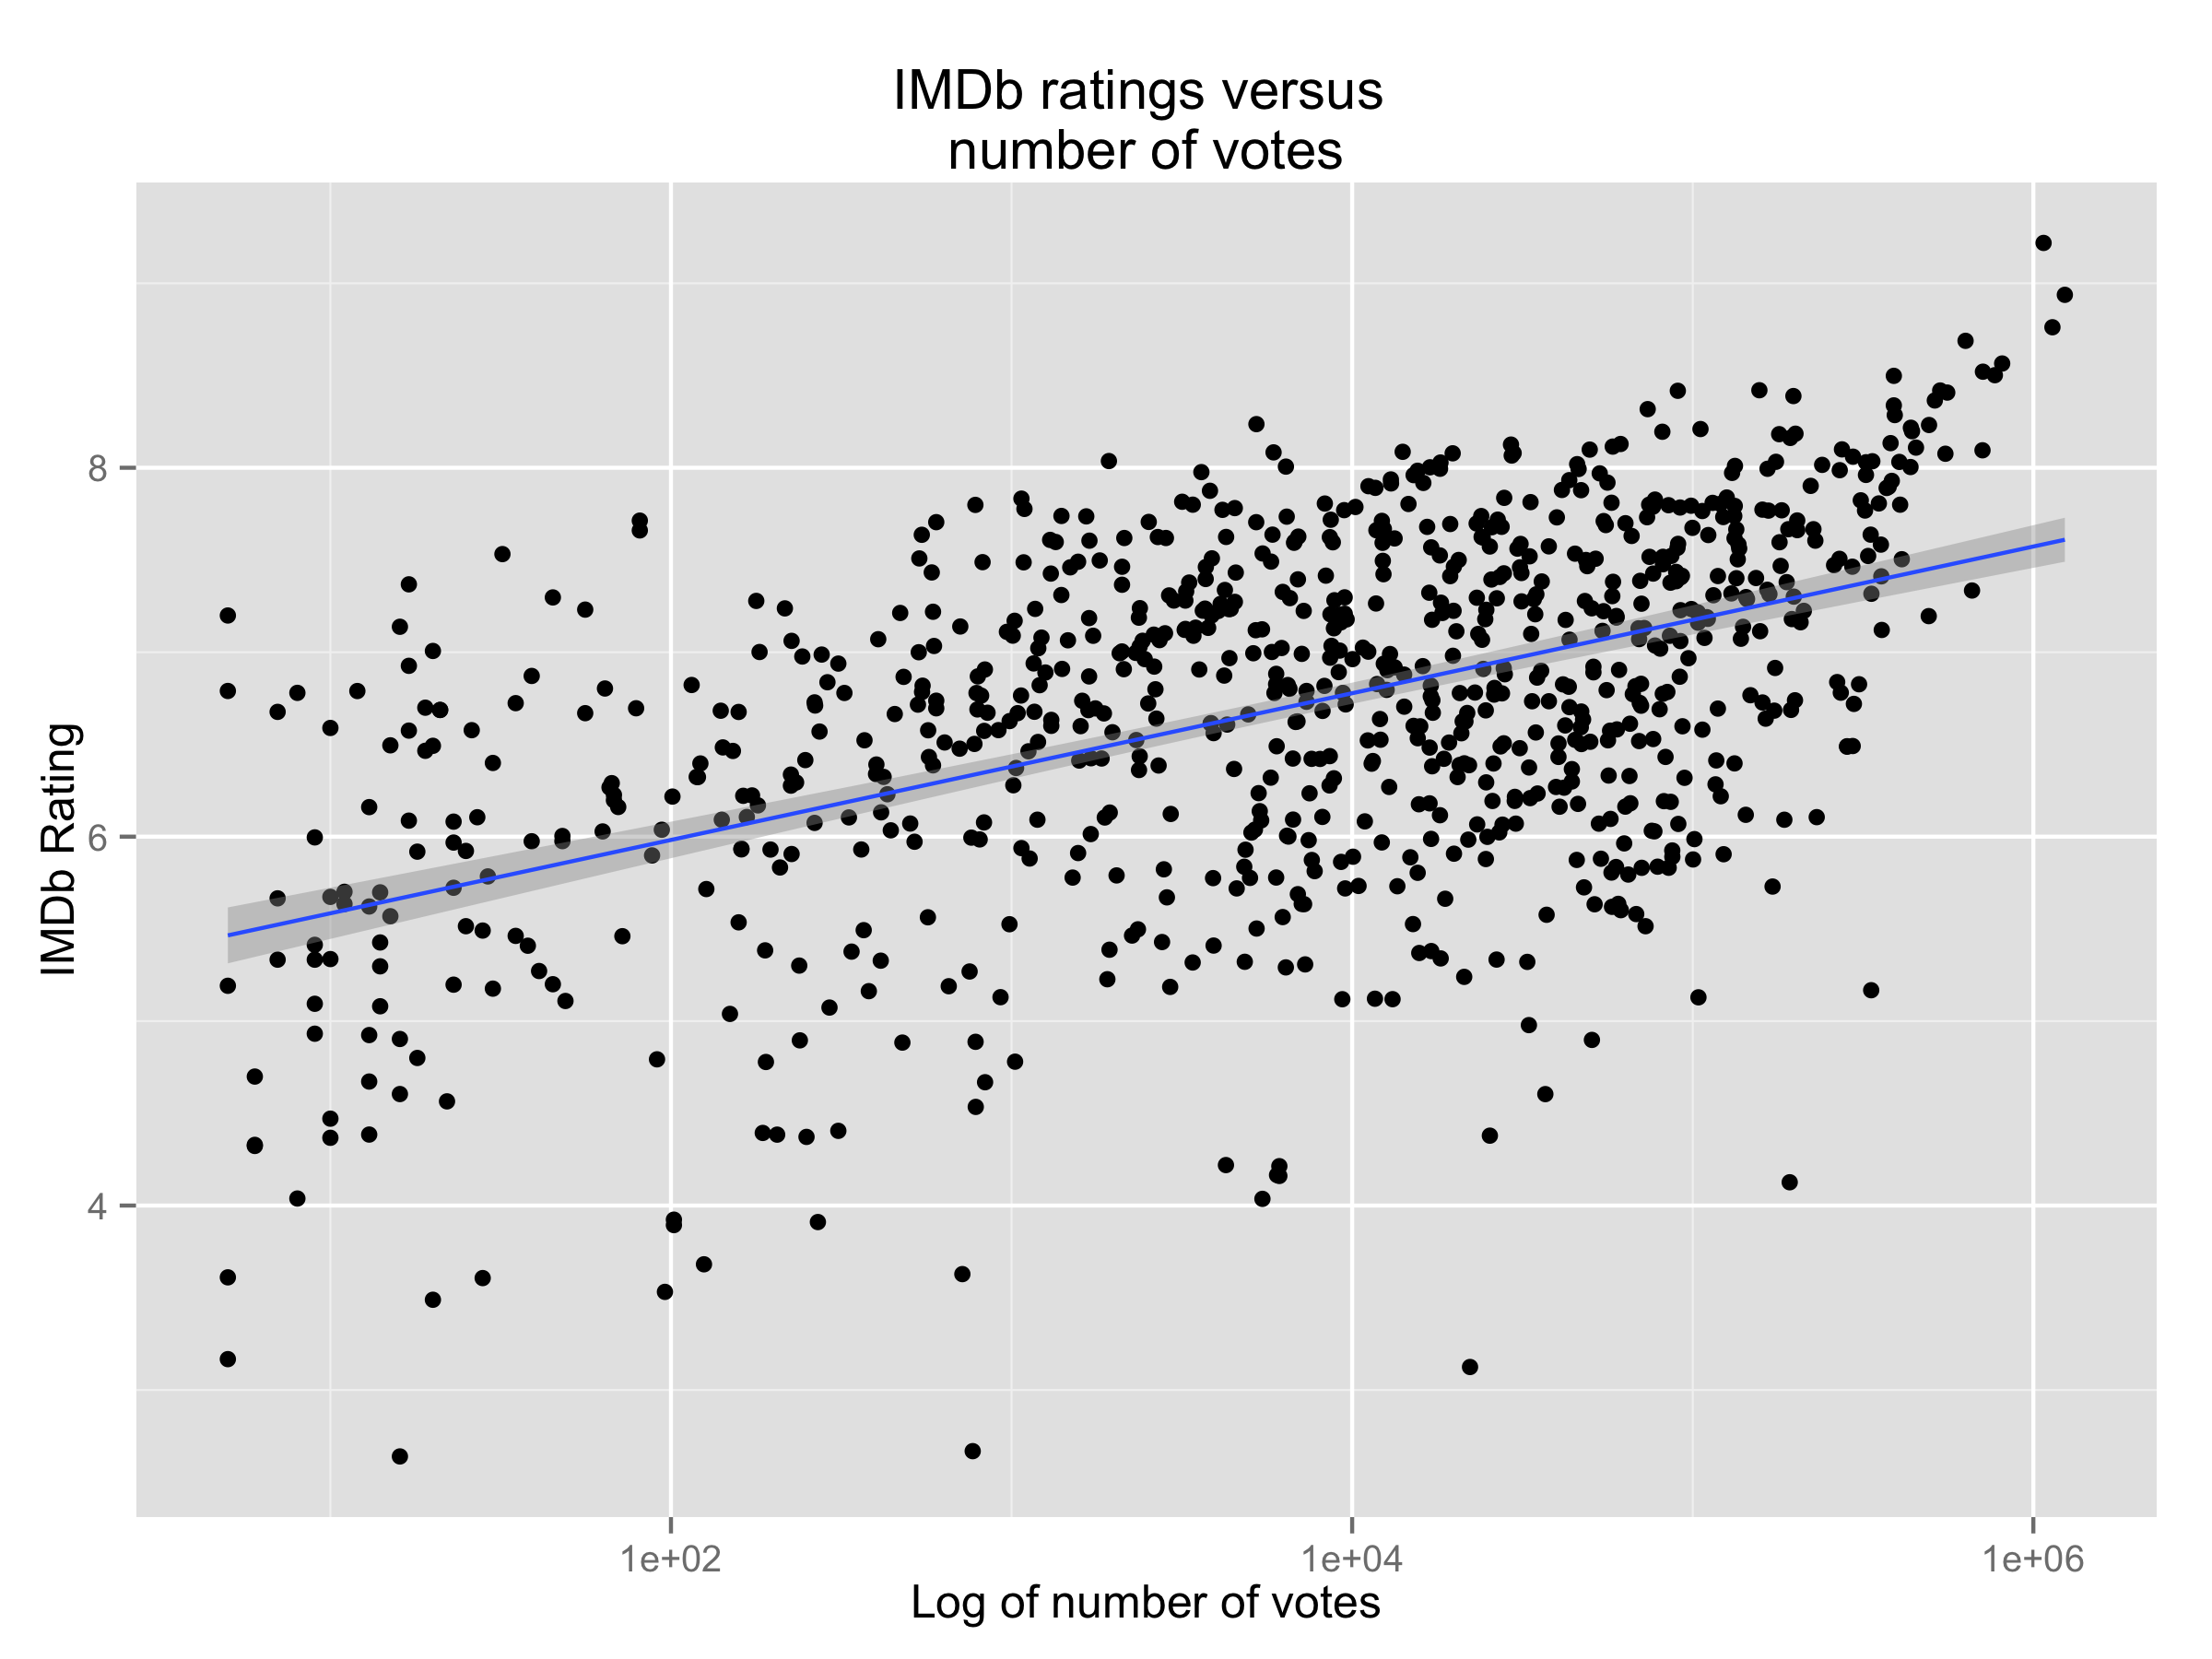
\includegraphics[scale=0.1]{ratingsimdb}
    \subcaption{IMDb}
    \label{fig:1b}
  \end{subfigure}
  \caption{Avereage rating compared to number of votes cast. We see an upwards trend in both}
  \label{fig:1}
\end{figure}

In their separate listing of top 250 movies, IMDb uses a so-called Bayesian average in ratings, taking into account the number of votes given. It is calculated as:
$$WR (\text{Weighted Ranking})=\frac{v}{v+m}R+\frac{m}{v+m}C$$
Where $R$ is the average rating for the movie, $v$ is the number of votes for the movie, $m$ is a minimum number required to be listed on the top 250 and $C$ is the mean rating for the report. 

We have considered using a Bayesian average in the model of IMDb in calculating average rated, as we have the data needed to do so. However, we stick to the original ratings. Under the Bayesian average, any rating with a number of votes given under an arbitrary number ie. 1000, will converge to the mean rating, and pull the ratings above the arbitrary number towards the mean in decreasing degree with the number of votes cast. This will give the figures in figure \ref{fig:1} a trumpet-like shape and give a large number of ratings the mean rating, destroying the ordinality that we are trying to examine. 

Even though the number of votes cast, intuitively should signal a greater weight or certainty about the rating, there are som biases that should be taken into account

Herding is in line with the data in figure \ref{fig:1}

Top movies are most exposed

\subsection{Ethics}




\end{document}


